\cleardoublepage

\chapter{Desarrollo Hardware}
\label{makereference5}

Una vez terminado el período de pruebas, ya con el kit de desarrollo nRF51-DK de Nordic como opción principal y con la placa XTRINSIC-SENSE-BOARD de Element 14, que incorpora el acelerómetro MMA84910 de 3 ejes, pudimos comenzar a desarrollar la parte hardware de este proyecto.

El desarrollo se centró en dos elementos: la \textbf{comunicación por I2C} entre la placa de desarrollo y el acelerómetro y el \textbf{envío de datos mediante Bluetooth Low Energy} desde la placa hacia un dispositivo móvil. A continuación se describirán los pasos realizados.

\section{Comunicación con el acelerómetro por I2C}
\label{makereference5.1}

El modelo nRF51-DK utiliza GPIO (General Purpose Input/Output), que son unos pines genéricos que pueden programarse como entrada o salida. Dos de estos pines se pueden configurar como un bus I2C, que se usa para comunicarse con una gran variedad de dispositivos externos, en este caso la placa XTRINSIC-SENSE-BOARD. 

I2C es un bus de datos con conexión serie síncrona unidireccional (half-duplex) que se puede dar de 2 tipos:
\begin{itemize}
	\item Maestro/Esclavo
	\item Esclavo/Maestro
\end{itemize}

\textbf{Maestro.} Inicia la transferencia generando las condiciones de inicio y parada de la señal de reloj. Transmite la dirección del esclavo y determina el sentido de la transferencia (lectura-escritura). La comunicación siempre la inicia el Master y el esclavo espera órdenes.\\

\textbf{Esclavo.} Este responde sólo cuando se dirigen a él. La temporización se controla mediante la línea de reloj del bus.\\

La transmisión de información se hace a través de 2 cables, uno para transmitir los datos (SDA) y otro para transmitir la señad del reloj (SCL). Otro cable para activar el acelerómetro (ENABLE) y otros 2 cables de toma de tierra (GND) y corriente (VDD) con este cablado tenemos conectado el sensor con la placa de desarrollo.

\begin{figure}[h]%t=top, b=bottom, h=here
	\centering
    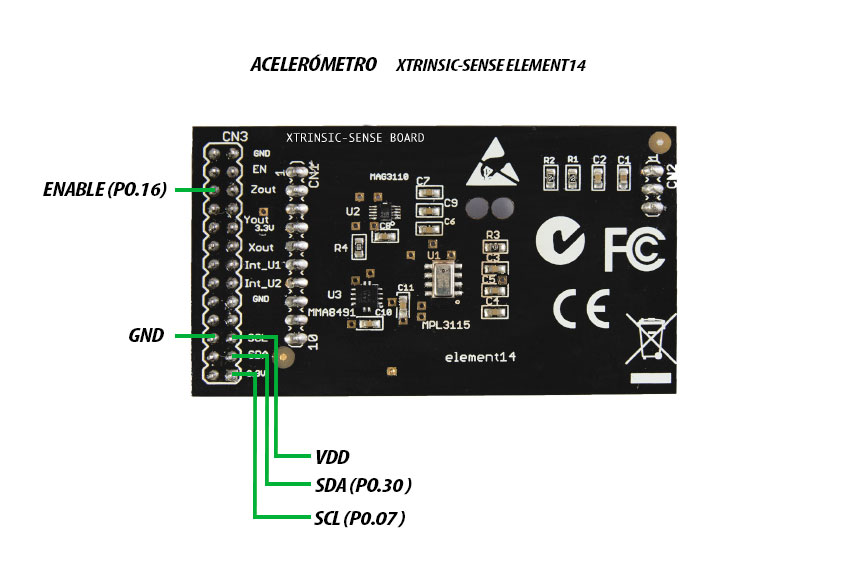
\includegraphics[scale=0.6]{figures/estructura_xtrinsic.jpg}
    \caption[Cableado del acelerómetro por I2C]{Cableado del acelerómetro por I2C}
   	\label{figuraXtrinsic}
\end{figure}

\subsection{Lectura de datos}
\label{makereference5.1.1}

El acelerómetro MMA8491Q tiene 7 registros donde se guardan los datos de acelerometría que han sido recogidos en la lectura. El primer registro es un registro de estado en el que se indica si alguno de los ejes ha cambiado desde la última muestra, los 6 registros siguientes dividen cada eje en los 8 bits más significativos y los 6 menos significativos, haciendo un total de 14 bits por eje. En la tabla que se muestra en la Figura~\ref{figuraRegistrosAcc} se puede observar la información de los 7 registros.

\begin{figure}[h]%t=top, b=bottom, h=here
	\centering
    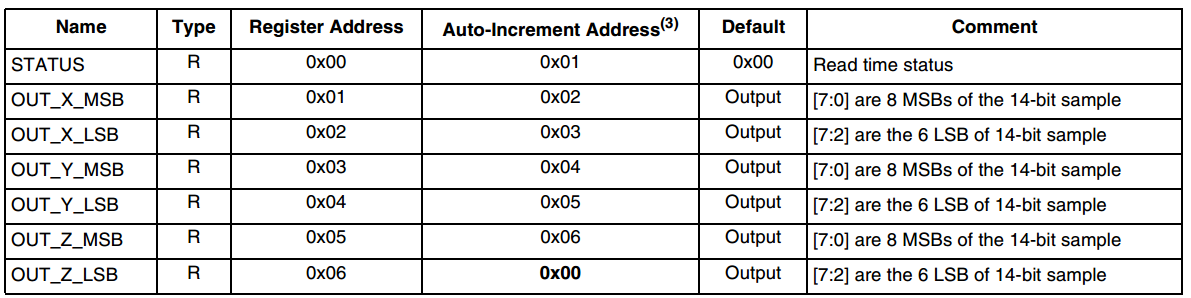
\includegraphics[width=\textwidth]{figures/registros_Acelerometro.png} % TODO hacer que esto no quede horrible
    \caption[Registros del acelerómetro]{Tabla con los registros del acelerómetro~\cite{DatasheetAcc}}
   	\label{figuraRegistrosAcc}
\end{figure}

Estos 14 bits se utilizan para especificar los valores de cada eje en un rango de +8000 mg a -8000 mg. Para ello utilizan el formato de la tabla que se puede ver en la Figura~\ref{figuraValoresAcc} sacada del datasheet~\cite{DatasheetAcc}. Se puede observar que se utiliza un Complemento a 2 para definir los números negativos. La forma de parsearlos se explicará más adelante.

\begin{figure}[h]%t=top, b=bottom, h=here
	\centering
    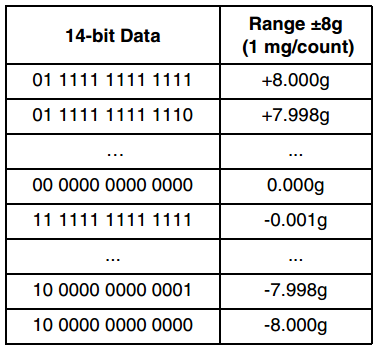
\includegraphics[scale=0.6]{figures/rango_datos_acelerometro.png} % TODO hacer que esto no quede horrible
    \caption[Rango de datos del acelerómetro]{Rango de datos del acelerómetro~\cite{DatasheetAcc}}
   	\label{figuraValoresAcc}
\end{figure}

El acelerómetro establece una serie de pasos para poder establecer la comunicación por I2C en el modo \textit{Multiple Byte Read}, que apunta al siguiente registro una vez concluida la lectura del anterior:

\begin{itemize}
	\item Se manda el comando Start condition con la dirección 0x55 y 1 bit de lectura-escritura a 0 para indicar escritura, el esclavo responde con una trama ACK.
	\item Se transmite la dirección del registro que se quiere leer y el esclavo manda una trama ACK.
	\item Se transmite el comando Repeated Start Condition con la dirección del acelerómetro, y esta vez el bit de lectura-escritura a 1 indicando lectura.
	\item El esclavo manda una trama ACK y transmite los datos del registro indicado.
	\item Por último, se transmite una trama ACK y una señal de stop para finalizar.
\end{itemize}

Una vez recibidos estos datos en la placa de Nordic, se juntan y se parsean siguiendo la siguiente fórmula:

\begin{lstlisting}[frame=single]

	WORD = (MSB << 6) | (LSB >> 2);
	
	if (WORD >= 0x2000)
		WORD -= 0x4000;

	NATURAL = (1000 * WORD + 512) >> 10;

\end{lstlisting}

Donde MSB es el byte con los bits más signigicativos, LSB es el byte con los bits menos significativos, y WORD y NATURAL son variables enteras. El resultado, de 14 bits, se guarda en una variable 16, que luego se dividirá en 2 bytes separados para poder enviarlos mediante Bluetooth.

Paso por paso, lo que hacemos es:

\begin{itemize}
	\item Concatenamos los dos grupos de bits leidos por separado del bus.
	\item Cambiamos el signo si es negativo, almacenandolo como un numero negativo de 16bits.
	\item Cambiamos la escala de -8192 / 8191 a -8000 / 8000
\end{itemize}

\subsection{Filtrado}
\label{makereference5.4.2}

En un entorno ideal, los datos que recoja el acelerómetro en un período en el que se encuentre estático deberían ser únicamente el valor de la gravedad (1g) repartido entre los 3 ejes, ya que es una aceleración constante que experimenta cualquier objeto en este planeta.

Lejos de ese caso, la información que recibimos varía ligeramente, normalmente en una escala de unos pocos mg. Para eliminar este ruido realizamos un filtrado consistente en recoger una muestra de 10 valores e insertarlos en un Búfer circular para poder filtrarlos a través de una media ponderada. El dar pesos a los datos permite que los últimos valores no se pierdan y que la media se actualice lo suficientemente rápido en caso de cambios bruscos.

\section{Comunicación Bluetooth}
\label{makereference5.2}

Como mencionábamos en el Capítulo~\ref{makereference2}, hemos elegido el Modo de Conexión para realizar el enlace y el intercambio de datos entre la placa de Nordic y el dispositivo móvil. En este caso tendremos los roles GAP y GATT (Explicados en las Secciones~\ref{makereference2.3.2} y~\ref{makereference2.4.1}, respectivamente) que se muestran en la Tabla~\ref{tablaRoles5}. 

El dispositivo móvil actúa como Central, ya que realiza el escaneo y la conexión, y como Cliente porque es el que envía las peticiones para recibir la información.

La placa nRF51-DK actúa como Periférico, pues manda paquetes de anuncio y acepta las conexiones entrantes, y como Servidor, al ser el que guarda la información y responde a las peticiones.

\begin{table}
	\begin{center}
	\begin{tabular}[c]{|c|c|c|}
        \hline
        & GAP & GATT \\
        \hline
        Dispositivo Móvil & Central & Cliente \\
    	\hline
    	Placa nRF51-DK & Periférico & Servidor \\
    	\hline
	\end{tabular}
    \caption{Roles GAP y GATT del dispositivo móvil y de la placa nRF51-DK}
    \label{tablaRoles5}
   \end{center}
\end{table}

Empezamos configurando el Perfil de Acceso Genérico (GAP) para establecer la información que incluyen los paquetes de anuncio:

\begin{itemize}
	\item El dispositivo es sólo BLE y no utiliza Bluetooth clásico.
	\item Se le permite a otros dispositivos su descubrimiento.
	\item La lista de servicios que contiene, en la que aparecerá el servicio mencionado anteriormente.
	\item El nombre del dispositivo, dado por una cadena de caracteres.
	\item El método de conexión.
\end{itemize}

Toda esta información estará disponible para cualquier dispositivo que se encuentre escaneando.\\

Seguidamente configuramos el Perfil de Atributo Genérico (GATT). Definimos el dispositivo como servidor GATT y, para encapsular los datos del acelerómetro, creamos un servicio con UUID 0xA000, al que le asignaremos una característica con UUID 0xA001. Esto se hace mediante las clases \textit{GattService} y \textit{GattCharacteristic} que nos ofrece la API de mbed. Estas clases permiten establecer los siguientes parámetros:

\textbf{Característica.} Le podemos definir un tamaño máximo y mínimo de los datos que van a contener, en nuestro caso siempre va a tener 6 bytes (3 ejes divididos en 2 bytes cada uno). También especificamos aquí que este valor es de sólo lectura.

\textbf{Servicio.} Le asignamos una lista en la que únicamente aparecerá nuestra característica.\\

Como se ha explicado en la Sección~\ref{makereference5.1.1}, los datos extraídos del acelerómetro se guardan en la nRF51-DK en tres variables de 16 bits, aunque la API BLE de mbed obliga a actualizar el valor de una característica utilizando un array de variables de 8 bits, por lo que necesitamos dividir los 16 bits de cada eje en dos bytes separados. Esto hace que el dispositivo móvil reciba la información también de este modo, por lo que se tienen que juntar de nuevo al recibirlos.
